\subsection{Matrix Calculus}

  There is nothing special about matrix calculus on its own, since matrices are themselves vectors; they can be sufficiently analyzed using vector calculus. Regardless, we will emphasize a few points. Let
  \begin{equation}
    A: \mathbb{R} \longrightarrow \text{Mat}(m \times n, \mathbb{R})
  \end{equation}
  be a matrix valued differential function. That is, the $m \times n$ component functions of $A$ is differentiable. Then, just like in calculus, we introduce differentiation rules.
  \begin{align*}
    & \frac{d}{d x} \big( A(t) + B(t)\big) = \frac{d}{d t} A(t) + \frac{d}{d t} B(t) \\
    & \frac{d}{d x} \big( c A(t)\big) = c \frac{d}{d t} A(t)
  \end{align*}
  The scalar multiplication can actually be extended. By linearity (of matrix multiplication), we can say that if $A$ is independent of $t$, then 
  \begin{equation}
    \frac{d}{d x} A B (x) = A \frac{d}{d x} B(x)
  \end{equation}
  The linearity of the derivative allows us to state more rules. Given that $v: \mathbb{R}^n \longrightarrow \mathbb{R}$ is a scalar valued function and $l \in (\mathbb{R}^n)^*$, then  
  \begin{equation}
    \frac{d}{d x} l \big( v(x) \big) = l \bigg( \frac{d}{d x} v(x) \bigg)
  \end{equation}
  This result can be extended to when $v$ is replaced by matrix valued function $A$ and $l$ is replaced by $\phi: \text{Mat}(m \times n, \mathbb{R}) \longrightarrow \mathbb{R}$. 
  \begin{equation}
    \frac{d}{d x} \phi \big( A(x) \big) = \phi \bigg( \frac{d}{d x} A(x) \bigg)
  \end{equation}
  Since the trace is a linear operator, we have the following theorem. 

  \begin{theorem}
    Given a linear function $A: \mathbb{R} \longrightarrow \text{Mat}(n, \mathbb{R})$ with paramater $x$, 
    \begin{equation}
      \frac{d}{d x} \Tr{A} = \Tr \bigg( \frac{d}{d x} A \bigg)
    \end{equation}
    Note that $A$ in here really means $A(x)$.
  \end{theorem}

  The product rule of matrix calculus is similar.
  \begin{equation}
    \frac{d}{d x} A B = \bigg(\frac{d}{d x} A\bigg) \cdot B + A \cdot \bigg(\frac{d}{d x} B \bigg)
  \end{equation}
  It is also noting that the derivative of the inner product of two vector valued functions $v, w: \mathbb{R} \longrightarrow \mathbb{R}^n$ is 
  \begin{equation}
    \frac{d}{d x} \big( v(x), w(x) \big) = \Big( \frac{d}{d x} v(x), w(x) \Big) + \Big( v(x), \frac{d}{d x} w(x) \Big)
  \end{equation}

  \begin{definition}
    A matrix valued function $A$ is \textbf{invertible at a point $x \in \mathbb{R}$} if there exists a function, denoted $A^{-1}$ such that
    \begin{equation}
      A(x) A^{-1} (x) = A^{-1}(x) A(x) = I
    \end{equation}
    where $I$ is the identity matrix. If there exists such $A^{-1}$ for all values $x \in \mathbb{R}$, then $A$ is said to be \textbf{invertible}. 
  \end{definition}

  \begin{theorem}
    Let $A$ be a matrix valued function, differentiable and invertible. Then, the function $A^{-1}$ is also differentiable and 
    \begin{equation}
      \frac{d}{d x} A^{-1} = - A^{-1} \bigg( \frac{d}{d x} A \bigg) A^{-1}
    \end{equation}
  \end{theorem}
  \begin{proof}
    We derive this using the product rule. 
    \begin{align*}
      0 = \frac{d}{d x} I & = \frac{d}{d x} \big( A(x) A^{-1} (x) \big) \\
      & = A(x) \bigg(\frac{d}{d x} A^{-1} (x) \bigg) + \bigg( \frac{d}{d x} A(x) \bigg) A^{-1} (x) \\
      \implies \frac{d}{d x} A^{-1} (x) & = - A^{-1} (x) \bigg( \frac{d}{d x} A(x) \bigg) A^{-1}(x)
    \end{align*}
  \end{proof}
  Note that the chain rule is a rule of differentiaion that applies for scalar valued functions. That is, given $f: V \longrightarrow \mathbb{R}$ and $g: \mathbb{R} \longrightarrow V$ ($V$ vector space), 
  \begin{equation}
    \frac{d}{d x} f \circ g (x) = f^\prime \big( g(x) \big) \cdot \frac{d}{d x} g(x)
  \end{equation}
  The $\cdot$ operation in the right hand side is the operation of multiplication in the field $\mathbb{R}$. But given $f: \text{Mat}(n, \mathbb{R}) \longrightarrow \mathbb{R}$ and $A \mathbb{R} \longrightarrow \text{Mat}(n, \mathbb{R})$, multiplication within the algebra of matrices are inherently different than component-wise operations, so the chain rule does not apply (it would apply if matrix multiplication was defined component-wise). 

  \begin{example}
    Let $f(A) \equiv A^2$, and let $A$ be a matrix valued function. Then, 
    \begin{align*}
      \frac{d}{d x} f \circ A(x) = \frac{d}{d x} \big( A(t) \big)^2 & = \bigg( \frac{d}{d x} A(x) \bigg) \cdot A(x) + A(x) \cdot \bigg( \frac{d}{d x} A(x) \bigg) \\
      & \neq 2 A(x) \cdot \frac{d}{d x} A(x)
    \end{align*}
    since matrix multiplication is in general not commutative. 
  \end{example}

  \begin{theorem}
    \begin{equation}
      \frac{d}{d x} A^k = A^\prime A^{k-1} + A A^\prime A^{k-2} + \cdots + A^{k-2} A^\prime A + A^{k-1} A^\prime
    \end{equation}
  \end{theorem}
  \begin{proof}
    We inductively apply the product rule
    \begin{equation}
      \frac{d}{d x} A^k = A^\prime A^{k-1} + A \frac{d}{d x} A^{k-1}
    \end{equation}
  \end{proof}

  \begin{corollary}
    Given any polynomial $p$ with $A$ a differentiable, square matrix valued function, if $A$ and $A^\prime$ commute, then 
    \begin{equation}
      \frac{d}{d x} p(A) = p^\prime (A) A^\prime
    \end{equation}
  \end{corollary}
  \begin{proof}
    We can completely define differentiation over the vector space of polynomials with the formula
    \begin{equation}
      \frac{d}{d x} A^k = k A^{k-1} A^\prime \; \forall k \in \mathbb{N}
    \end{equation}
  \end{proof}

  \begin{corollary}
    Given polynomial $p$ with $A$ a differentiable, square matrix valued function, 
    \begin{equation}
      \frac{d}{d x} \Tr{p(A)} = \Tr{\big( p^\prime(A) \cdot A^\prime \big)}
    \end{equation}
  \end{corollary}
  \begin{proof}
    Use the cyclic trace property.
  \end{proof}

  \begin{definition}
    The \textbf{exponential map} is defined
    \begin{equation}
      \text{exp}: \text{Mat}(n, \mathbb{C}) \longrightarrow \text{Mat}(n, \mathbb{C})
    \end{equation}
    where 
    \begin{equation}
      e^A = I + A + \frac{1}{2!} A^2 + \frac{1}{3!} A^3 + \cdots = \sum_{k=0}^\infty \frac{1}{k!} A^k
    \end{equation}
    where $A^0 \equiv I$. This can clearly be extended to when $A$ is a square, matrix valued function. 
  \end{definition}

  This final theorem establishes the connection between the determinant and trace. 

  \begin{theorem}
    Given a differentiable square matrix valued function $A$ such that $A$ is invertible for a certain $x \in \mathbb{R}$, then 
    \begin{equation}
      \frac{d}{d x} \log{\det{A}} = \Tr \bigg( A^{-1} \frac{d}{d x} A \bigg)
    \end{equation}
    Where the log mapping is the inverse of the exponential mapping of matrices. 
  \end{theorem}

  \begin{definition}
    The \textbf{commutator} in the algebra of $n \times n$ matrices is defined as 
    \begin{equation}
      [A, B] = A B - B A
    \end{equation}
  \end{definition}

  \begin{theorem}
    If $A$ and $B$ are commuting square matrices, then 
    \begin{equation}
      e^{A + B} = e^A \, e^B
    \end{equation}
    In general, the solution $C$ to the equation
    \begin{equation}
      e^{A} \, e^B = e^C
    \end{equation}
    is given by the \textbf{Baker-Campbell-Hausdorff formula}, defined
    \begin{equation}
      C = A + B + \frac{1}{2}[A,B] + \frac{1}{12} [A,[A,B]] - \frac{1}{12} [B,[A,B]] + \ldots
    \end{equation}
    consisting of terms involving higher commutators of $A$ and $B$. The full series is much too complicated to write, so we ask the reader to be satisfied with what is shown. 
  \end{theorem}

  \begin{corollary}
    \begin{equation}
      \Tr{\log{e^A \, e^B}} = \Tr{A} + \Tr{B}
    \end{equation}
  \end{corollary}

\subsection{Stochastic Matrices}

  \begin{definition}[Entrywise Positive]
    A real $n \times n$ matrix $P$ is \textbf{entrywise positive} if all entries are positive real numbers. We similarly define entrywise positive vectors having components as positive real numbers. With this notion of positiveness. We can define
    \begin{equation}
      A > B \iff A - B > 0 \iff (A-B)_{i j} > 0 \; \forall i, j
    \end{equation}
  \end{definition}

  Note that this definition of positive matrices is \textit{not} the same as positive-definite matrices! 

  \begin{theorem}[Perron's Theorem]
    Every entrywise positive matrix $P$ has a real \textbf{dominant eigenvalue}, denoted $\lambda(P) \in \mathbb{R}$ satisfying
    \begin{enumerate}
      \item $\lambda(P) > 0$, and the associated eigenvector $h >0$
      \item $\lambda(P)$ is a simple eigenvalue
      \item every other eigenvalue $\kappa$ satisfies: $|\kappa| < \lambda(P)$
      \item there is no other eigenvector $\geq 0$, i.e. all other eigenvectors have at least 1 negative entry.
    \end{enumerate}
  \end{theorem}

  \begin{definition}[Stochastic Matrix]
    A \textbf{stochastic matrix} is a matrix $A$ where the elements of each column $a_i$ sum up to $1$. $A$ is \textbf{doubly stochastic} if $A$ and $A^T$ are stochastic. 
  \end{definition}

  \begin{theorem}
    Let $S > 0$ be a positive stochastic matrix. Then, $\lambda(S) = 1$. Furthermore, given any nonnegative vector $x \geq 0$, 
    \begin{equation}
      \lim_{N \rightarrow \infty} S^N x = c h
    \end{equation}
    where $h$ is the dominant eigenvector and $c$ is some positive constant. 
  \end{theorem}

  A common application of this theorem likes in probability and statistics. Since nonnegative stochastic matrices can be used to represent discrete-time Markov Chains, with the dominant eigenvector representing the stationary distribution $\pi$. 

  Another application lies within defining Google's Page Rank Algorithm. Upon representing a page as a node, if there is one link that directs the user from page $A$ to page $B$, we can represent this as an oriented path from node $A$ to node $B$. Given that we have $n$ nodes, we can construct a $n \times n$ matrix $A$ where 
  \begin{equation}
    a_{i j} \equiv  \frac{\text{number of paths from node $i$ to node $j$}}{\text{number of nonzero entries in $j$th column}}
  \end{equation}

  \begin{figure}[H]
    \centering
    \begin{subfigure}[b]{0.48\textwidth}
      \centering
      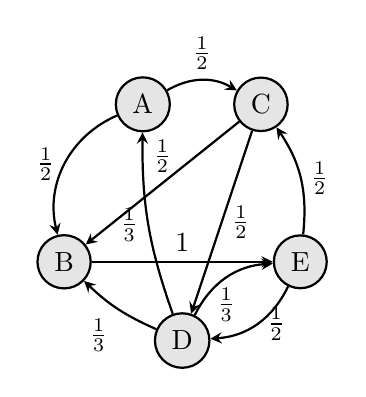
\begin{tikzpicture}[
        scale=0.5,
        ->,
        >=stealth,
        node distance=4cm,
        thick,
        main node/.style={circle, draw, fill=black!10, minimum size=4mm}
        ]

        % Nodes/States
        \node[main node] (A) at (0,4) {A};
        \node[main node] (B) at (-2,0) {B};
        \node[main node] (C) at (3,4) {C};
        \node[main node] (D) at (1,-2) {D};
        \node[main node] (E) at (4,0) {E};

        % Edges with reversed direction
        % From A to B (curving outwards)
        \path (A) edge [bend right=40] node[left] {$\frac{1}{2}$} (B);
        \path (A) edge [bend left=30] node[above] {$\frac{1}{2}$} (C);
        
        % From B to other states
        \path (C) edge node[above] {$\frac{1}{2}$} (B);
        \path (D) edge [bend left=10] node[below left] {$\frac{1}{3}$} (B);
        \path (D) edge [bend left=10] node[left] {$\frac{1}{3}$} (A);
        
        % From E to C (corrected direction)
        \path (E) edge [bend right=20] node[right] {$\frac{1}{2}$} (C);
        
        % From D to other states
        \path (C) edge  node[right] {$\frac{1}{2}$} (D);
        \path (D) edge [bend left=30] node[below] {$\frac{1}{3}$} (E);
        
        % From E to other states
        \path (B) edge node[above] {$1$} (E);
        \path (E) edge [bend left=30] node[right] {$\frac{1}{2}$} (D);
      \end{tikzpicture}
    \end{subfigure}
    \hfill 
    \begin{subfigure}[b]{0.48\textwidth}
      \centering
      \begin{equation}
        \begin{pmatrix}0&0&0&\frac{1}{3}&0\\
        \frac{1}{2}&0&\frac{1}{2}&\frac{1}{3}&0\\
        \frac{1}{2}&0&0&0&\frac{1}{2}\\
        0&0&\frac{1}{2}&0&\frac{1}{2}\\
        0&1&0&\frac{1}{3}&0\end{pmatrix}
      \end{equation}
    \end{subfigure}
    \caption{Markov chain graph and corresponding adjacency/transition matrix.}
    \label{fig:markov_chain}
  \end{figure}

  However, the theorem above requires the matrix to be strictly positive, which is often not true for Markov chains in general. This theorem does not hold true in the following example, 
  \begin{equation}
    A = \begin{pmatrix}
    0&0&0&\frac{1}{3} \\
    \frac{1}{2}&0&0&\frac{1}{3} \\
    0&0&0&\frac{1}{3} \\
    \frac{1}{2}&0&0&0
    \end{pmatrix} \implies A^{1000} 
        \begin{pmatrix}
    \frac{1}{4} \\ \frac{1}{4} \\ \frac{1}{4} \\ \frac{1}{4}
    \end{pmatrix} = 
        \begin{pmatrix}
    0 \\ 9/20 \\ 11/20 \\ 0
    \end{pmatrix}, \; A^{1001} 
        \begin{pmatrix}
    \frac{1}{4} \\ \frac{1}{4} \\\frac{1}{4} \\ \frac{1}{4}
    \end{pmatrix} = 
        \begin{pmatrix}
    0 \\ 11/20 \\ 9/20 \\ 0
    \end{pmatrix}
  \end{equation}
  That is, $A^N v$ oscillates between these two values. Furthermore, given three notes $A, B, C$ as such

  \begin{figure}[H]
    \centering 
    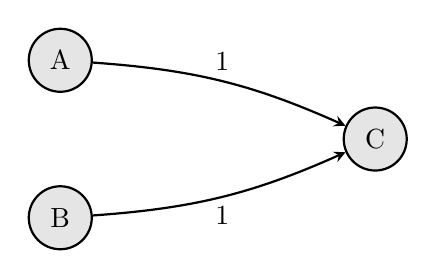
\begin{tikzpicture}[
      ->,
      >=stealth,
      node distance=3cm,
      thick,
      main node/.style={circle, draw, fill=black!10, minimum size=8mm}
      ]
      % Nodes
      \node[main node] (A) at (0,2) {A};
      \node[main node] (B) at (0,0) {B};
      \node[main node] (C) at (4,1) {C};

      % Edges with weight labels
      \path (A) edge [bend left=10] node[above] {$1$} (C);
      \path (B) edge [bend right=10] node[below] {$1$} (C);
    \end{tikzpicture}
    \label{fig:degenerate_markov_chain}
  \end{figure}
  the entries of the adjacency matrix is not well-defined. 
  \begin{equation}
     \begin{pmatrix} 0&0&? \\0&0&? \\1&1&?\end{pmatrix}
  \end{equation}
  Google CEO Larry Page actually developed a solution by implementing what he called a \textit{dampening factor}. Given stochastic matrix $B_{i j} = \frac{1}{N}$, he redefined the chain to be 
  \begin{equation}
    M = \alpha A + (1-\alpha) B, \; 0< \alpha < 1
  \end{equation}
  It is clear that $M$ is now a strictly positive stochastic matrix. The $\alpha$ is the dampening factor, and its optimal value is known to be about $0.67$. The value of the alpha determines how much of the data is "washed away." When $\alpha = 0$, none of the data is lost, and when $\alpha = 1$, all of the data is lost. 

  Due to the limitations of Perron's theorem, we can extend it with the following.

  \begin{theorem}[Frobenius Extension to Perron]
    Any $n \times n$ matrix $F \geq 0$, $F \neq 0$ has eigenvalue $\lambda$ such that
    \begin{enumerate}
      \item $\lambda \geq 0$ and $F h = \lambda h$, $h\geq 0$ \item every eigenvalue $\kappa$ satisfies: $|\kappa| \leq \lambda$ 
      \item if $|\kappa| = \lambda$, then 
      \begin{equation}
        \kappa = e^{\frac{2 \pi i k}{m}} \lambda, \; k, m \in \mathbb{Z}_+, \; m \leq n
      \end{equation}
    \end{enumerate}
  \end{theorem}

